
\documentclass[dvipdfmx]{jsarticle}
\usepackage[T1]{fontenc}
\usepackage[dvipdfmx]{hyperref}
\usepackage{lmodern}
\usepackage{latexsym}
\usepackage{amsfonts}
\usepackage{amssymb}
\usepackage{mathtools}
\usepackage{nccmath}
\usepackage{amsthm}
\usepackage{multirow}
\usepackage{graphicx}
\usepackage{wrapfig}
\usepackage{here}
\usepackage{float}
\usepackage{ascmac}
\usepackage{url}
\def\NO{01}
\def\LECTURENAME{論理と計算}
\begin{document}
\title{\LECTURENAME{}:第\NO{}回演習問題}

\author{5419045 高林 秀}

\date{}
\maketitle

\begin{itemize}
\item Latexを用いて作成し,PDF形式で提出してください
\end{itemize}


\vspace*{\baselineskip}

\begin{enumerate}\setlength{\itemsep}{\baselineskip}

\item
  講義資料で示したもの以外で,
  日常生活の中で行っている演繹・発想・帰納推論の各具体例を挙げ,
  それらがなぜ演繹・発想・帰納推論と言えるのか,それぞれ説明しなさい.
\paragraph{解答}\par
\begin{itemize}
  \item 演繹:(例)「食べ物を買うにはお金が必要(買うという行為はお金を支払う必要がある)」、「人が生きるなら食べ物が必要(人間は動物、動物は食べ物を食べないと生きていけない)」ならば「人が生きるにはお金が必要」
  \begin{itemize}
    \item 理由:現代社会において「食べ物を買うにはお金がかかる」と「人間ならば食べ物を食べる」の2条件は真である。第2条件の人間ならば食べ物を食べるにある、「食べ物」はお金を支払うことで手に入れることができる、と第1条件で定められている。したがって、結論の「人が生きるにはお金が必要」は真。このとき、前提条件A{「食べ物を買うにはお金が必要」、「人が生きるなら食べ物が必要」}が普遍的事実であり真であることから、結論B{「人が生きるにはお金が必要」}を導出しているので演繹推論である。
  \end{itemize}
  \item 帰納:(例)「保健の授業で視力を悪くする習慣について学習した」、「友人Aは夜中暗い部屋で毎日長時間ビデオゲームをしていて、視力が落ちたそうだ」、「新聞にある眼科の医師のインタビュー記事で、暗い部屋で画面との距離が近い状態を長時間保ちながら、テレビゲームやスマートフォンなど強い光を放つものを視界に入れると視力が段々と落ちてしまう、と報道されていた。」という事があった。したがって「暗い部屋でテレビゲームなどの強い光を長時間視界に入れると視力が落ちる」。
   \begin{itemize}
    \item 理由:複数の具体的な事例を統合して、共通する傾向や共通点である「暗い部屋でテレビゲームなどの強い光を長時間視界に入れると視力が落ちる」というルールを導いている。したがって帰納推論である。
  \end{itemize}
  \item 発想:(例)「インフルエンザ」ならば「高熱である」。なので高熱ならばインフルエンザである、
  \begin{itemize}
    \item 理由:「高熱である」という結論から「インフルエンザ」というケースを導出できるので発想推論である。
  \end{itemize}
\end{itemize}
\item
  講義資料のオントロジーを用いた論理推論の例において,
  Elizabethの子孫をすべて見つけなさい.
  また,合わせて子孫と推論できる理由を説明しなさい.
  %
  なお,子孫を表す関係を``hasDescendants''と表記し,
  ``hasAncestor''と反対(inverseOf)の関係にあるものとする.
  \paragraph{解答}\par
  \begin{itemize}
    \item Charles
    \item William
    \item Henry
  \end{itemize}
  \paragraph{理由}図から、Eizabeth "hasChild" Charlesであることが示されているので、Charlesが子孫に該当する。図よりWilliam "hasFather" Charlesである。このとき、Williamの父親がCharlesであるので、Charlesの凝っ共はWiliamであり。したがってCharles "hasChild" Williamも真である。このことから "hasChild"で関係を結ぶと「Elizabeth→Charles→William」となるので、Williamも子孫に該当する。加えて図からWiliam "hasBrother" Henryであることが示されているので、Henry "hasFather" Charlesも真である。したがって、Charles "hasChild" Henryも真である。すなわち、→の関係を"hasDescendants"とすると「Elizabeth→Charles→William, Henry」となる。導出課程は下図。
  \begin{figure}[H]
    \centering
    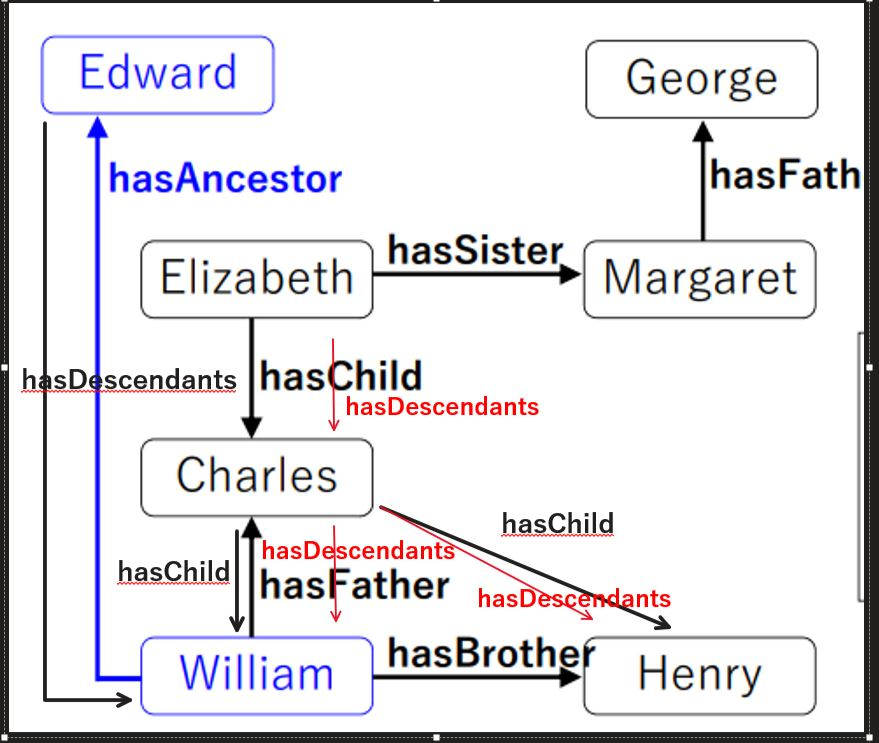
\includegraphics[scale=0.4]{cap1.JPG}
  \end{figure}

\item
  講義資料のWumpus worldの例において,
  例題の通り[1,1]→[2,1]→[1,1]→[1,2]→[2,2]→[2,3]と動き,
  [2,3]で知覚 [Stench, Breeze, Glitter, None, None]を得たときに
  初めてわかる事実(新事実)をすべて示しなさい.
  %
  また各新事実が,どの様なルール(規則)と既知の事実を用いて導出されるのか詳細に示しなさい.
\paragraph{解答}
\begin{itemize}
  \item 新事実:黄金の山を発見、獣はまだ殺されていない、周囲に壁はない、$[2,4],[1,3],[2,2],[3,3]$のいずれかに獣がいる、$[2,3]$は安全、$[2,4],[1,3],[2,2],[3,3]$のいずれかに穴がある。
  \item 導出課程\par
  まず、「黄金の山を発見」は知覚情報Glitterより、Glitterは黄金のある部屋のみで知覚されるので、導出される。「獣はまだ殺されていない、周囲に壁はない」は、知覚情報bumpとscreamがNoneであることより、人間はまだ獣を殺しておらず、壁には衝突していない、と導出される。「$[2,4],[1,3],[2,2],[3,3]$のいずれかに獣がいる」は、知覚情報strenchより、$[2,3]$から上下左右隣の範囲に獣が存在していることが導出される。したがって、screamがNoneであることも考慮すると、獣はまだ生きている。「$[2,4],[1,3],[2,2],[3,3]$のいずれかに穴がある。」は、知覚情報breezeより、$[2,3]$から上下左右隣の範囲に穴が存在していることが導出される。
\end{itemize}

\end{enumerate}
\end{document}
